
\section{The Electrical and Gravitational Forces\footnote{
1990-93 Dept. of Physics and Astronomy, Dickinson College. Supported by FIPSE
(U.S. Dept. of Ed.) and NSF. Portions of this material have been modified locally
and may not have been classroom tested at Dickinson College.
} }

Name \rule{2.0in}{0.1pt}\hfill{}Section \rule{1.0in}{0.1pt}\hfill{}Date \rule{1.0in}{0.1pt}

\begin{quote}
I began to think of gravity extending to the orb of the moon, and . . . I deduced
that the forces which keep the planets in their orbs must be reciprocally as
the squares of their distances from the centers about which they revolve: and
thereby compared the force requisite to keep the moon in her orb with the force
of gravity at the surface of the earth, and found them to answer pretty nearly.
All this was in the two plague years of 1665 and 1666, for in those days I was
in the prime of my age for invention, and minded mathematics and philosophy
more than at any time since. --- Isaac Newton 
\end{quote}
\textbf{Objective }

To understand the similarities of the gravitational and electrical forces. 

\textbf{Overview }

The enterprise of physics is concerned ultimately with mathematically describing
the fundamental forces of nature. Nature offers us several fundamental forces,
which include a strong force that holds the nuclei of atoms together, a weak
force that helps us describe certain kinds of radioactive decay in the nucleus,
the force of gravity, and the electromagnetic force. 

\textit{Two kinds of force dominate our everyday reality: 
the gravitational force
acting between masses and the Coulomb force acting between electrical charges.}
The gravitational force allows us to describe mathematically how objects near
the surface of the earth are attracted toward the earth and how the moon revolves
around the earth and planets revolve around the sun. The genius of Newton was
to realize that objects as diverse as falling apples and revolving planets are
both moving under the action of the same gravitational force. 

\vspace{0.3cm}
{\par\centering 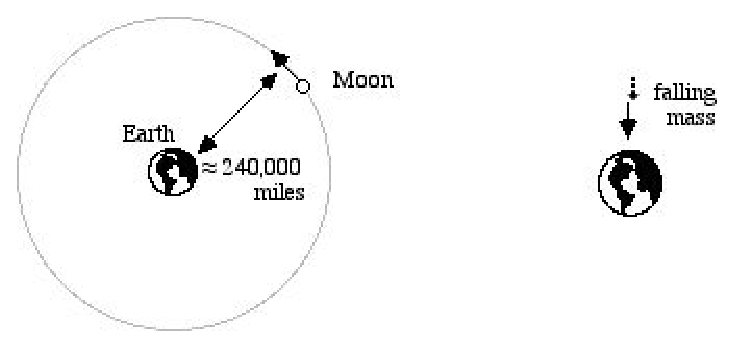
\includegraphics{elec_grav_fig1.eps} \par}
\vspace{0.3cm}

Similarly, the Coulomb force allows us to describe how one charge ``falls''
toward another or how an electron orbits a proton in a hydrogen atom. 

\vspace{0.3cm}
{\par\centering 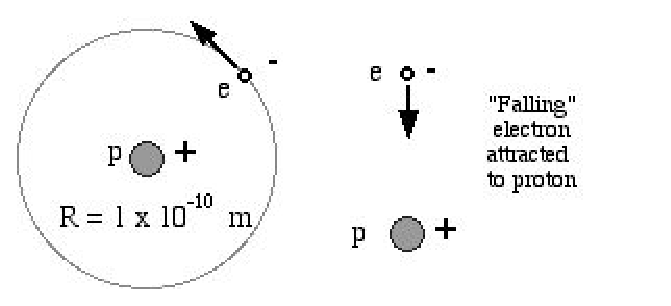
\includegraphics{elec_grav_fig2.eps} \par}
\vspace{0.3cm}

The fact that both the Coulomb and the gravitational forces lead to objects
falling and to objects orbiting around each other suggests that these forces
might have the same mathematical form. 

In this unit we will explore the mathematical symmetry between electrical and
gravitational forces for two reasons. First, it is beautiful to behold the unity
that nature offers us as we use the same type of mathematics to predict the
motion of planets and galaxies, the falling of objects, the flow of electrons
in circuits, and the nature of the hydrogen atom and of other chemical elements.
Second, what you have already learned about the influence of the gravitational
force on a mass can be applied to aid your understanding of the forces on charged
particles. 

\textbf{Activity 1: Comparison of Electrical and Gravitational Forces }

Let's start our discussion of this comparison with the familiar expression of
the Coulomb force exerted on charge 1 by charge 2. 

\vspace{0.3cm}
{\par\centering 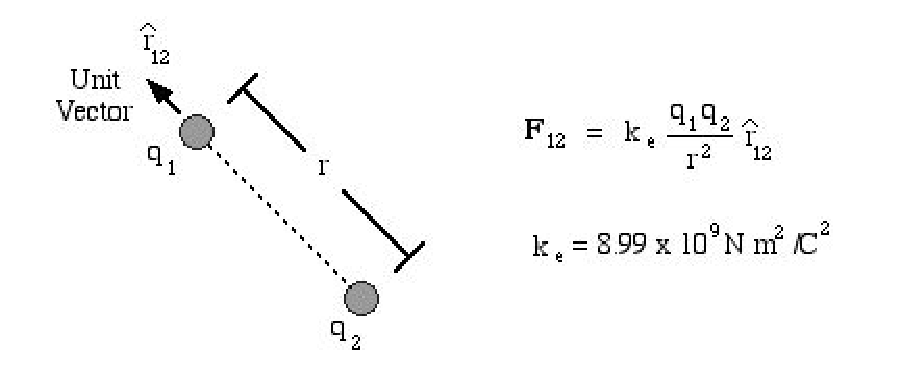
\includegraphics{elec_grav_fig3.eps} \par}
\vspace{0.3cm}

Charles Coulomb did his experimental investigations of this force in the 18th
century by exploring the forces between two small charged spheres. Much later,
in the 20th century, Coulomb's law enabled scientists to design cyclotrons and
other types of accelerators for moving charged particles in circular orbits
at high speeds. 

Newton's discovery of the universal law of gravitation came the other way around.
He thought about orbits first. This was back in the 17th century, long before
Coulomb began his studies. A statement of Newton's universal law of gravitation
describing the force experienced by mass 1 due to the presence of mass 2 is
shown below in modern mathematical notation: 

\vspace{0.3cm}
{\par\centering 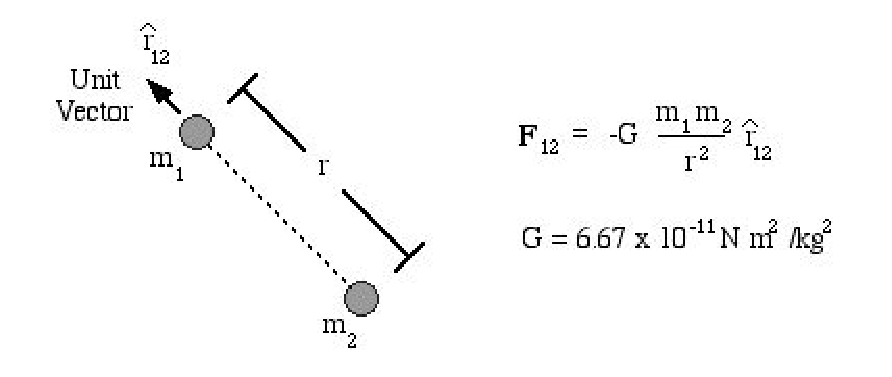
\includegraphics{elec_grav_fig4.eps} \par}
\vspace{0.3cm}

About the time that Coulomb did his experiments with electrical charges in the
18th century, one of his contemporaries, Henry Cavendish, did a direct experiment
to determine the nature of the gravitational force between two spherical masses
in a laboratory. This confirmed Newton's gravitational force law and allowed
him to determine the gravitational constant, $G$. A fact emerges that is quite
amazing. Both types of forces, electrical and gravitational, are very similar.
Essentially the same mathematics can be used to describe orbital and linear
motions due to either electrical or gravitational interactions of the tiniest
fundamental particles or the largest galaxies. This statement needs to be qualified
a bit when electrons, protons and other fundamental particles are considered.
A new field called quantum mechanics was developed in the early part of the
last
century to take into account the wave nature of matter, which we don't actually
study in introductory physics. However, even in wave mechanical calculations
electrical forces like those shown above are used. 

\textbf{Activity 2: The Electrical vs. the Gravitational Force} 

Examine the mathematical expression for the two force laws.

(a) What is the same about the two force laws?
\vspace{20mm}

(b) What is different? For example, is the force between two like masses attractive
or repulsive? How about two like charges? What part of each equation determines
whether the like charges or masses are attractive or repulsive?
\vspace{20mm}

(c) Do you think negative mass could exist? If there is negative mass, would
two negative masses attract or repel?
\vspace{20mm}

\textbf{Which Force is Stronger-- Electrical or Gravitational?} 

Gravitational forces hold the planets in our solar system in orbit and account
for the motions of matter in galaxies. Electrical forces serve to hold atoms
and molecules together. If we consider two of the most common fundamental particles,
the electron and the proton, how do their electrical and gravitational forces
compare with each other?

Let's peek into the hydrogen atom and compare the gravitational force on the
electron due to interaction of its mass with that of the proton to the electrical
force between the two particles as a result of their charge. In order to do
the calculation you'll need to use some well known constants.

Electron: \(m_{e}  = 9.1 \times 10^{-31} \) kg, \( q_{e}  = - 1.6 
\times 10^{-19} \)
C 

Proton: \( m_{p}  = 1.7 \times 10^{-27} \) kg, \( q_{p}  = +1.6 \times 10^{-19} \)
C 

Distance between the electron and proton: \(r = 0.530 \times 10^{-10} \) m

\textbf{Activity 3: The Electrical vs. the Gravitational Force in the Hydrogen
Atom}

(a) Calculate the magnitude of the electrical force on the electron. Is it attractive
or repulsive?
\vspace{20mm}

(b) Calculate the magnitude of the gravitational force on the electron. Is it
attractive or repulsive?
\vspace{20mm}

(c) Which is larger? By what factor (i.e., what is the ratio)?
\vspace{20mm}

(d) Which force are you more aware of on a daily basis? If your answer does
not agree with that in part (c), explain why.
\vspace{20mm}

\textbf{Activity 4: The Gravitational Force of the Earth}

(a) Use Newton's law of universal gravitation to show that the magnitude of the acceleration due to gravity on an object of mass m at a height h above the surface of the earth is given by the following expression.
\[
\frac{GM_{e}}{\left( R_{e}+h\right) ^{2}}\]


Hint: Because of the spherical symmetry of the Earth you can treat the mass
of the Earth as if it were all concentrated at a point at the Earth's center.
\vspace{40mm}

(b) Calculate the acceleration due to gravity of a mass m at the surface of
the earth (h=0). The radius of the earth is \( R_{e}  \approx   6.38
\times 10^{3} \) km and its mass \( M_{e}  \approx  5.98 \times 10^{24} \)
kg. Does the result look familiar? How is this acceleration related to the gravitational
acceleration $g$?
\vspace{40mm}

(c) Use the equation you derived in part (a) to calculate the acceleration due
to gravity at the ceiling of the room you are now in. How does it differ from
the value at the floor? Can you measure the difference in the lab using the
devices available?
\vspace{30mm}

(d) Suppose you travel halfway to the moon. What is the new value of the acceleration due to gravity (neglecting the effect of the moon's pull)?  (Recall that the earth-moon distance is about 384,000 km.)
\vspace{30mm}

(e) Is the gravitational acceleration ``constant,'' $g$, really
a constant? Explain.
\vspace{30mm}

(f) In part (d) you showed that there is a significant gravitational attraction
halfway between the earth and the moon. Why, then, do astronauts experience ``weightlessness'' when they are orbiting a mere 120 km above the earth?

